\documentclass[11pt]{article}

\usepackage[utf8]{inputenc}
\usepackage[T1]{fontenc}
\usepackage{lmodern}
\usepackage[a4paper,portrait,margin=1.0cm]{geometry}
\usepackage{tikz}
\usepackage{xcolor}

% --- Colours ----------------------------------------------------------
\definecolor{crimson}{HTML}{B5121B}   % Lancaster crimson
\definecolor{plenbg}{HTML}{EEB8B8}    % plenary
\definecolor{talkbg}{HTML}{FBEEEE}    % regular talk
\definecolor{postbg}{HTML}{FBE2BD}    % spotlight / poster
\definecolor{brkbg}{HTML}{ECECEC}     % break
\definecolor{logbg}{HTML}{E3E9F0}     % logistics (lunch, dinner, remarks)

% --- Grid geometry ----------------------------------------------------
\def\hh{1.75}     % cm per hour (vertical scale; taller than landscape)
\def\cw{5.6}      % column width (cm)
\def\gap{0.35}    % gap between columns (cm)
\def\tw{5.1cm}    % text width inside a block
\def\gridr{17.65} % right end of the hour gridlines

% --- Content formatters ----------------------------------------------
\newcommand{\Talk}[2]{{\footnotesize\textbf{#1}}\\[-3pt]{\tiny\itshape\textcolor{gray}{#2}}}
\newcommand{\Plen}[2]{{\tiny\bfseries\color{crimson}PLENARY}\\[-3pt]{\footnotesize\textbf{#1}}\\[-3pt]{\tiny\itshape\textcolor{gray}{#2}}}
\newcommand{\Sess}[1]{{\footnotesize\bfseries #1}}
\newcommand{\Logi}[1]{{\scriptsize #1}}
\newcommand{\Tin}[1]{{\tiny #1}}
\newcommand{\Brk}{{\tiny\textcolor{gray}{Break}}}

% --- Block: xleft, tstart(h since 9am), tend, fill, time, content ----
% Narrow columns: the time sits on its own line above the content
% instead of in the top-right corner as in the landscape version.
\newcommand{\blk}[6]{%
  \fill[#4,draw=black!20,line width=0.3pt,rounded corners=1.5pt]
     ({#1},{-#2*\hh}) rectangle ({#1+\cw},{-#3*\hh});
  \node[anchor=north west,align=left,inner sep=2.5pt,text width=\tw]
     at ({#1},{-#2*\hh}) {{\tiny\textcolor{gray}{#5}}\\[-2.5pt]#6};
}

% --- Compact block: time and content on ONE line ---------------------
% For very short slots (10--15 min), where a stacked time line would
% push the text past the bottom edge and under the following block.
\newcommand{\blkc}[6]{%
  \fill[#4,draw=black!20,line width=0.3pt,rounded corners=1.5pt]
     ({#1},{-#2*\hh}) rectangle ({#1+\cw},{-#3*\hh});
  \node[anchor=north west,align=left,inner sep=2.5pt,text width=\tw]
     at ({#1},{-#2*\hh}) {{\tiny\textcolor{gray}{#5}}\ \ {\tiny #6}};
}

\setlength{\parindent}{0pt}
\pagestyle{empty}

\begin{document}

\begin{center}
  {\large\bfseries\color{crimson} MARS Annual Symposium 2026}\\[2pt]
  {\footnotesize Computational Mathematics and Probabilistic Machine Learning}\\[1pt]
  {\footnotesize Lancaster University \quad\textbullet\quad 9--11 September 2026}\\[1pt]
  {\scriptsize\color{gray} Draft programme --- 35-minute talks}
\end{center}
\vspace{-0.3em}

\begin{center}
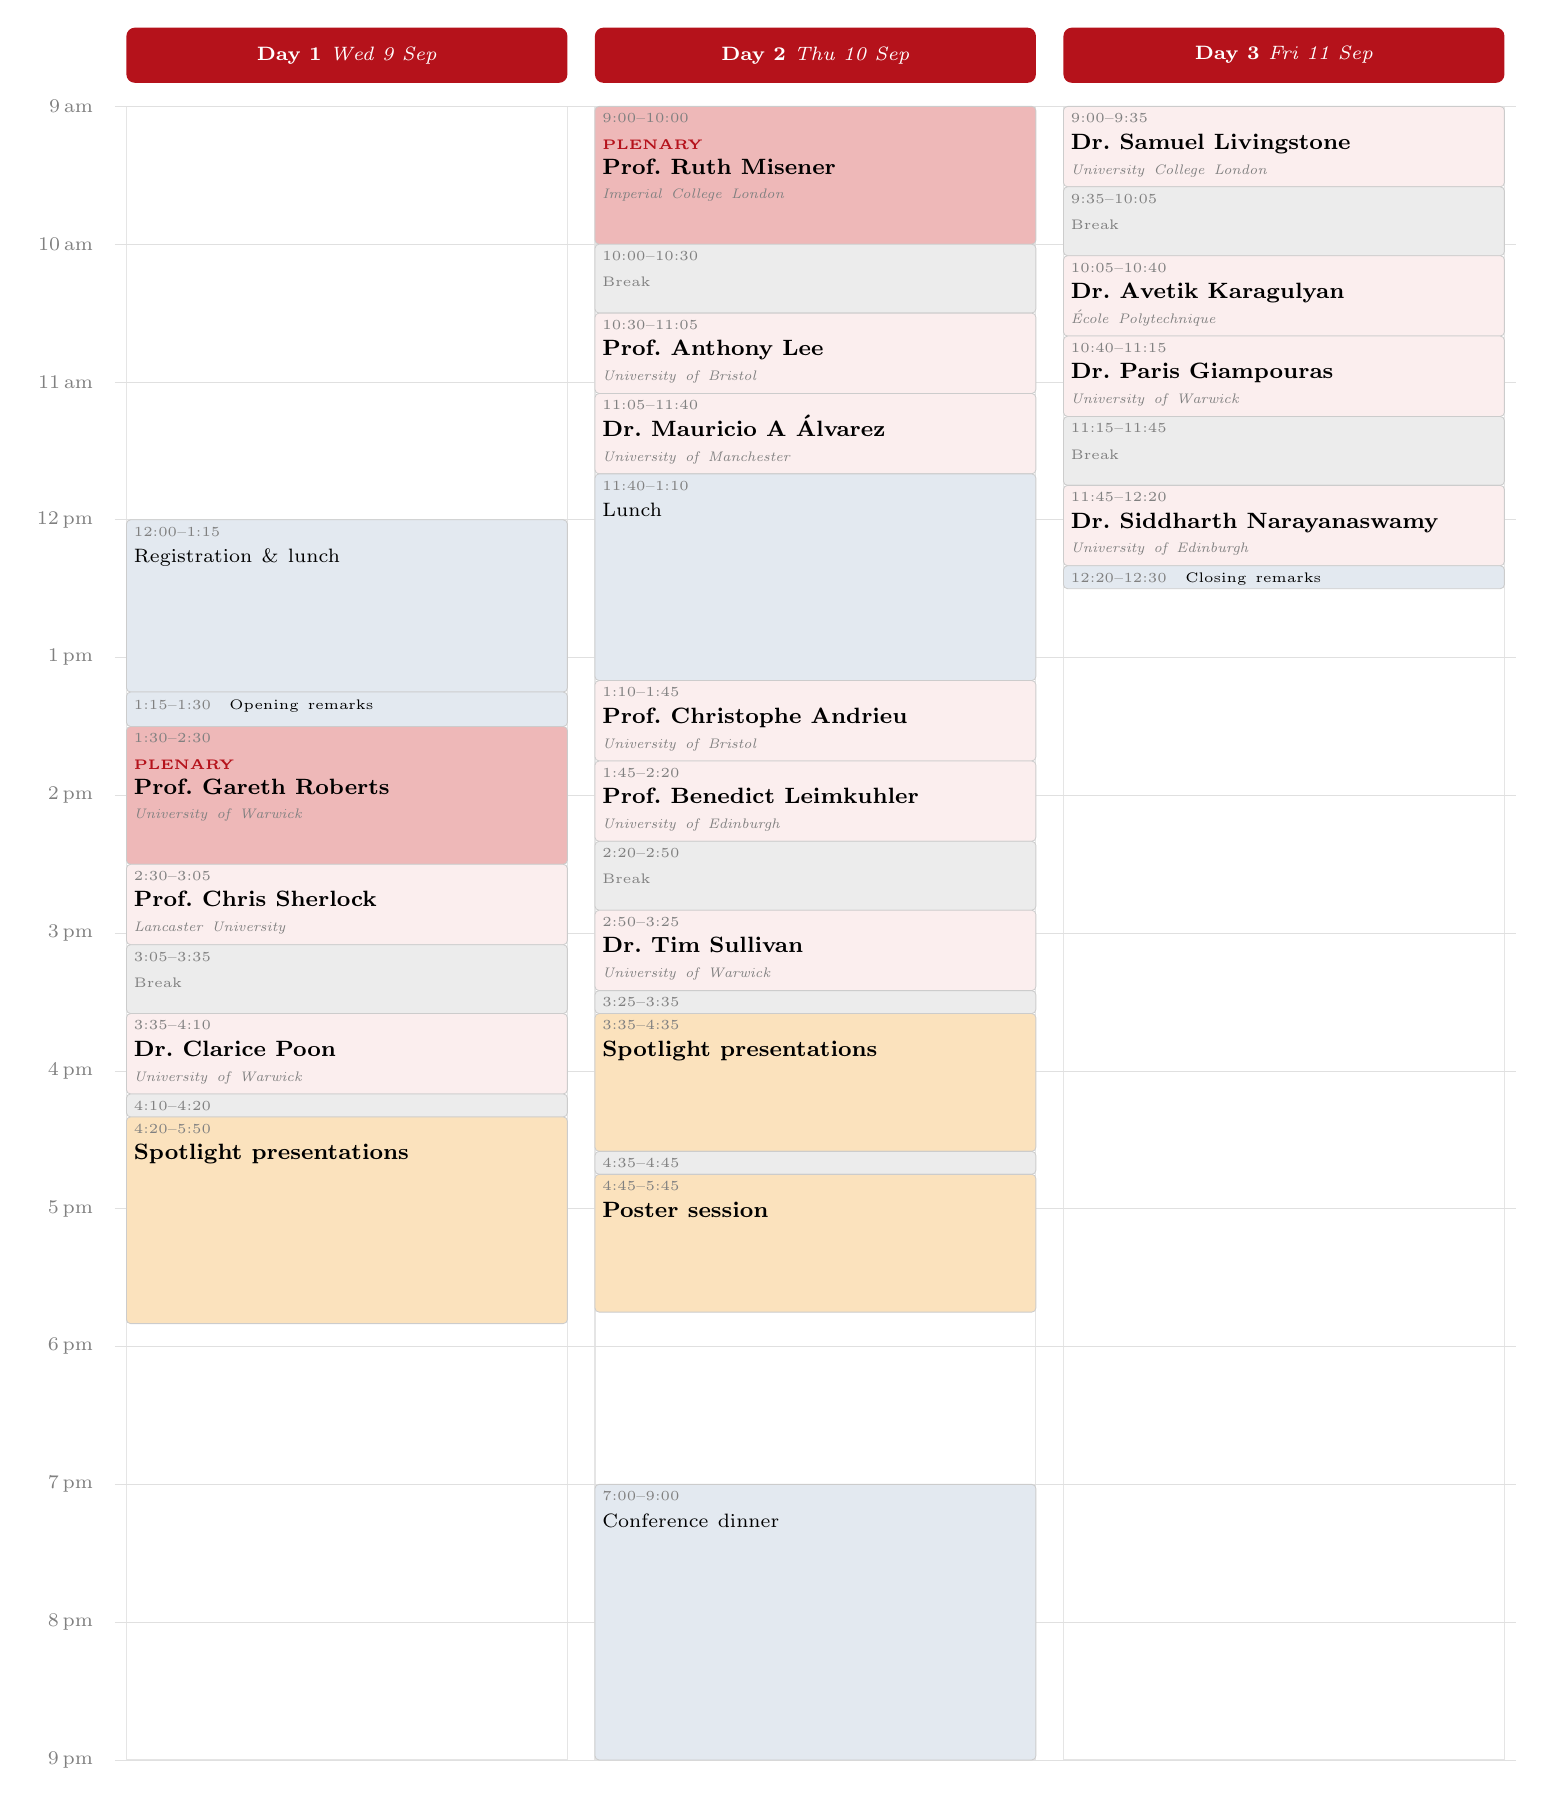
\begin{tikzpicture}

% --- column background frames ---------------------------------------
\foreach \x in {0,5.95,11.9}{
  \draw[black!10] ({\x},0) rectangle ({\x+\cw},{-12*\hh});
}

% --- hour gridlines + time labels -----------------------------------
\foreach \t/\lab in {0/{9\,am},1/{10\,am},2/{11\,am},3/{12\,pm},4/{1\,pm},%
5/{2\,pm},6/{3\,pm},7/{4\,pm},8/{5\,pm},9/{6\,pm},10/{7\,pm},11/{8\,pm},12/{9\,pm}}{
  \draw[black!12,line width=0.3pt] (-0.15,{-\t*\hh}) -- (\gridr,{-\t*\hh});
  \node[anchor=east,font=\scriptsize,text=gray] at (-0.3,{-\t*\hh}) {\lab};
}

% --- day header bars -------------------------------------------------
\foreach \x/\d in {0/{Day 1 {\normalfont\itshape Wed 9 Sep}},%
5.95/{Day 2 {\normalfont\itshape Thu 10 Sep}},%
11.9/{Day 3 {\normalfont\itshape Fri 11 Sep}}}{
  \fill[crimson,rounded corners=3pt] ({\x},0.3) rectangle ({\x+\cw},1.0);
  \node[text=white,font=\bfseries\scriptsize] at ({\x+0.5*\cw},0.65) {\d};
}

% ===================== DAY 1 (x = 0) ================================
\blk{0}{3.0}{4.25}{logbg}{12:00--1:15}{\Logi{Registration \& lunch}}
\blkc{0}{4.25}{4.5}{logbg}{1:15--1:30}{Opening remarks}
\blk{0}{4.5}{5.5}{plenbg}{1:30--2:30}{\Plen{Prof.\ Gareth Roberts}{University of Warwick}}
\blk{0}{5.5}{6.0833}{talkbg}{2:30--3:05}{\Talk{Prof.\ Chris Sherlock}{Lancaster University}}
\blk{0}{6.0833}{6.5833}{brkbg}{3:05--3:35}{\Brk}
\blk{0}{6.5833}{7.1667}{talkbg}{3:35--4:10}{\Talk{Dr.\ Clarice Poon}{University of Warwick}}
\blk{0}{7.1667}{7.3333}{brkbg}{4:10--4:20}{}
\blk{0}{7.3333}{8.8333}{postbg}{4:20--5:50}{\Sess{Spotlight presentations}}

% ===================== DAY 2 (x = 5.95) =============================
\blk{5.95}{0}{1}{plenbg}{9:00--10:00}{\Plen{Prof.\ Ruth Misener}{Imperial College London}}
\blk{5.95}{1}{1.5}{brkbg}{10:00--10:30}{\Brk}
\blk{5.95}{1.5}{2.0833}{talkbg}{10:30--11:05}{\Talk{Prof.\ Anthony Lee}{University of Bristol}}
\blk{5.95}{2.0833}{2.6667}{talkbg}{11:05--11:40}{\Talk{Dr.\ Mauricio A \'Alvarez}{University of Manchester}}
\blk{5.95}{2.6667}{4.1667}{logbg}{11:40--1:10}{\Logi{Lunch}}
\blk{5.95}{4.1667}{4.75}{talkbg}{1:10--1:45}{\Talk{Prof.\ Christophe Andrieu}{University of Bristol}}
\blk{5.95}{4.75}{5.3333}{talkbg}{1:45--2:20}{\Talk{Prof.\ Benedict Leimkuhler}{University of Edinburgh}}
\blk{5.95}{5.3333}{5.8333}{brkbg}{2:20--2:50}{\Brk}
\blk{5.95}{5.8333}{6.4167}{talkbg}{2:50--3:25}{\Talk{Dr.\ Tim Sullivan}{University of Warwick}}
\blk{5.95}{6.4167}{6.5833}{brkbg}{3:25--3:35}{}
\blk{5.95}{6.5833}{7.5833}{postbg}{3:35--4:35}{\Sess{Spotlight presentations}}
\blk{5.95}{7.5833}{7.75}{brkbg}{4:35--4:45}{}
\blk{5.95}{7.75}{8.75}{postbg}{4:45--5:45}{\Sess{Poster session}}
\blk{5.95}{10.0}{12.0}{logbg}{7:00--9:00}{\Logi{Conference dinner}}

% ===================== DAY 3 (x = 11.9) =============================
\blk{11.9}{0}{0.5833}{talkbg}{9:00--9:35}{\Talk{Dr.\ Samuel Livingstone}{University College London}}
\blk{11.9}{0.5833}{1.0833}{brkbg}{9:35--10:05}{\Brk}
\blk{11.9}{1.0833}{1.6667}{talkbg}{10:05--10:40}{\Talk{Dr.\ Avetik Karagulyan}{\'Ecole Polytechnique}}
\blk{11.9}{1.6667}{2.25}{talkbg}{10:40--11:15}{\Talk{Dr.\ Paris Giampouras}{University of Warwick}}
\blk{11.9}{2.25}{2.75}{brkbg}{11:15--11:45}{\Brk}
\blk{11.9}{2.75}{3.3333}{talkbg}{11:45--12:20}{\Talk{Dr.\ Siddharth Narayanaswamy}{University of Edinburgh}}
\blkc{11.9}{3.3333}{3.5}{logbg}{12:20--12:30}{Closing remarks}

\end{tikzpicture}
\end{center}

\vspace{-0.2em}
\begin{center}\scriptsize\color{gray}
\setlength{\fboxsep}{2pt}%
\colorbox{plenbg}{\phantom{XX}}~Plenary \quad
\colorbox{talkbg}{\phantom{XX}}~Talk (35\,min) \quad
\colorbox{postbg}{\phantom{XX}}~Spotlight / poster \\[3pt]
\colorbox{brkbg}{\phantom{XX}}~Break \quad
\colorbox{logbg}{\phantom{XX}}~Meals / remarks
\end{center}

\end{document}
